% !TEX root = ./Vorlesungsmitschrift AGLA 2.tex  
\lecture{Di 30.06. 10:15}{}

\begin{proof}[Beweis von \thref{projektive_quadriken_hauptachsenform}]
  Sei \( K \) ein Körper mit \( \characteristic-{K}\neq 2 \), \( A\in \sqmatrices{(n+1)}{K} \) eine symmetrische Matrix und
  \begin{equation*}
    Q=\Set{(x_0:\dotsc:x_n)\in \projectionspaceover{n}{K}|\transpose{\underline{x}}A\underline{x}=0}.
  \end{equation*}
  Sei \( s\maps K^{n+1}\times K^{n+1}\to K \) die durch \( s(\underline{x},\underline{y})\definedas \transpose{\underline{x}}A\underline{y} \) definierte symmetrische Bilinearform. Nach \thref{symmetrische_bilinearform_diagonalisierung} existiert eine Basis \( v_0,\dotsc,v_n \) von \( K^{n+1} \) mit 
  \begin{equation*}
    \transpose{\underline{v}_i}A\underline{v}_j=s(v_i,v_j)=0\quad i\neq j\logicspace  0\leq i,j\leq n.
  \end{equation*}
  \begin{proofdescription}
    \item[Fall \( K=\reals \)] Nach Permutation der Indizes \( 0\leq i\leq n \) können wir annehmen, dass es ganze Zahlen \( -1\leq k\leq m\leq n \) gibt mit
    \begin{equation*}
      \transpose{v_i}A v_i=\begin{cases}
        >0 & 0\leq i\leq k\\
        <0 & k+1\leq i\leq m\\
        =0 & m+1\leq i\leq n.
      \end{cases}
    \end{equation*}
    Setze
    \begin{equation*}
      \underline{w}_i\definedas \begin{cases}
        \frac{1}{\sqrt{\abs{\transpose{v_i}Av_i}}}v_i&0\leq i\leq m\\
        v_i & m+1\leq i\leq n.
      \end{cases}
    \end{equation*}
    Definiere eine Matrix \( S\in \invertiblematrices{n+1}{K} \) durch \( \inverse{S}=(\underline{w}_0,\dotsc,\underline{w}_n) \). Dann induziert \( S \) einen Isomorphismus \( F\maps K^{n+1}\to K^{n+1} \) und die Projektivität \( f=\projectionmap{} \) hat die Eigenschaft
    \begin{equation*}
      f(Q)=\Set{(y_0:\dotsc:y_n)\in \projectionspaceover{n}{K}|y_0^2+\dotsb+y_k^2-y_{k+1}^2-\dotsb-y_m^2=0}.
    \end{equation*}
    \item[Fall \( K=\complexs \)] Nach Permutation der Indizes \( 0\leq i \leq n \) können wir annehmen, dass es eine ganze Zahl \( -1\leq m\leq n \) gibt mit
    \begin{equation*}
      \transpose{v_i}Av_i=\begin{cases}
        \neq 0&0\leq i\leq m\\
        =0&m<i\leq n.
      \end{cases}
    \end{equation*}
    Wähle \( \lambda_i\in \fieldwithoutzero{C} \), \( 0\leq i \leq m  \), mit
    \begin{equation*}
      \lambda_i^2\p[\big]{\braceannotate{\neq 0}{\transpose{v_i}Av_i}}=1.
    \end{equation*}
    Setze
    \begin{equation*}
      \underline{w}_i=\begin{cases}
        \lambda_i v_i & 0\leq i\leq m\\
        v_i &m<i\leq n.
      \end{cases}
    \end{equation*}
    Definiere wie oben
    \begin{equation}
      \inverse{S}=\definedas(\underline{w}_0,\dotsc,\underline{w}_n)\in \invertiblematrices{n+1}{\complexs}.
    \end{equation}
    Die zu pNiceMatrixS  gehörende Koordinatentransformation hat dann die Eigenschaft
    \begin{equation*}
      f(Q)=\Set{(y_0:\dotsc:y_n)\in \projectionspaceover{n}{\complexs}|y_0^2+\dotsb+y_m^2=0}.
    \end{equation*}
  \end{proofdescription}
\end{proof}
\thref{symmetrische_bilinearform_diagonalisierung} ist auch für Körper \( K\neq \reals,\complexs \) nützlich.
\begin{beispiel*}
  Sei \( p \) eine Primzahl \( \neq 2 \) und \( K=\quotient{\wholes}{p\wholes} \). Betrachte eine Quadrik \( Q\subseteq \projectionspaceover{n}{K} \) gegeben durch
  \begin{equation*}
    Q=\Set{(x_0:\dotsc:x_n)\in \projectionspaceover{n}{K}|\transpose{\underline{x}}A\underline{x}=0}
  \end{equation*}
  mit einer symmetrischen Matrix
  \begin{equation*}
    A\in \sqmatrices{n+1}{\quotient{\wholes}{p\wholes}}.
  \end{equation*}
  Nach \thref{symmetrische_bilinearform_diagonalisierung} gibt es ein Koordinatentransformation
  \begin{equation}
    f\maps \projectionspaceover{n}{\quotient{\wholes}{p\wholes}}\to\projectionspaceover{n}{\quotient{\wholes}{p\wholes}},
  \end{equation}
  sodass
  \begin{equation*}
    f(Q)=\Set{(y_0:\dotsc:y_n)\in \projectionspaceover{n}{K}|\transpose{\underline{y}}D\underline{y}=0}
  \end{equation*}
  mit einer Diagonalmatrix
  \begin{equation*}
    D=\begin{pNiceMatrix} \beta_0 &  & 0 \\  & \Ddots &  \\ 0 &  & \beta_n \end{pNiceMatrix},
  \end{equation*}
  \( \beta_i\in K \), \( 0\leq i\leq n \). Sei \( \Gamma=\set{x^2|x\in \fieldwithoutzero{K}}\subseteq \fieldwithoutzero{K} \). Dann ist \( \abs{\Gamma}=\frac{p-1}{2} \), denn die Abbildung
  \begin{align*}
    \fieldwithoutzero{K}&\to \Gamma\\
    x&\mapsto x^2
  \end{align*}
  ist ein Gruppenhomomorphismus mit Kern \( \Set{\pm 1} \) und induziert eine Bijektion
  \begin{equation*}
    \fieldwithoutzero{K}\setminus\Set{\pm 1}\to \Gamma.
  \end{equation*}
  In der Matrix \( D \) können wir die Indizes so umordnen, dass es ganze Zahlen \( -1\leq k\leq m\leq n \) gibt mit
  \begin{equation*}
    \beta \begin{cases}
      \in \Gamma &0\leq i\leq k\\
      \in \fieldwithoutzero{K}\setminus \Gamma & k+1\leq i\leq m\\
      =0 &m+1\leq i\leq n.
    \end{cases}
  \end{equation*}
  Für \( 0\leq i\leq k \) wähle \( \lambda_i\in \fieldwithoutzero{K} \) mit \( \beta_i=\lambda_i^2 \). Sei \( r\in \fieldwithoutzero{K}\setminus \Gamma \). Für \( k+1\leq i\leq m\) wähle \( \lambda_i\in K \) mit \( \beta_i=r\lambda_i^2 \). Setze
  \begin{align*}
    y_i&\definedas \inverse{\lambda_i}z_i\quad 0\leq i\leq m\\
    y_i&\definedas z_i\quad m<i\leq n.
  \end{align*}
  Nach Anwendung dieser Koordinatentranformation hat die Quadrik \( Q \) die Form
  \begin{equation*}
    \Set{(z_0:\dotsc:z_n)\in \projectionspaceover{n}{K}|z_0^2+\dotsb+z_k^2+r(z_{k+1}^2+\dotsb+z_m^2)=0}.
  \end{equation*}
\end{beispiel*}
\file{Projektive Quadriken Teil 3}
\begin{bemerkung*}
  In \thref{projektive_quadriken_hauptachsenform} können wir jede Quadrik \( Q\subseteq \projectionspaceover{n}{\reals} \) nach einer Koordinatentranformation auf eine der Formen
  \begin{equation*}
    \tag{\( * \)}\label{reduzierte_projektive_quadrik}x_0^2+\dotsb+x_k^2-x_{k+1}^2-\dotsb-x_m^2=0
  \end{equation*}
  mit \( -1\leq k\leq m\leq n \) reduzieren.

  Unterschiedliche Polynome \eqref{reduzierte_projektive_quadrik} können die gleiche Quadrik \( Q \) beschreibe. Sei \( -1\leq m\leq n \) fest und \zb führt dann \( k=m \) auf 
  \begin{align*}
    Q&=\Set{(x_0:\dotsc:x_n)\in \projectionspaceover{n}{\reals}|x_0^2+\dotsb+x_m^2=0}\\
    &=\Set{(x_0:\dotsc:x_n)\in \projectionspaceover{n}{\reals}|x_0=\dotsb=x_m=0}\\
    &=\Set{(x_0:\dotsc:x_n)\in\projectionspaceover{n}{\reals}|-x_0^2-\dotsb-x_m^2=0},
  \end{align*}
  dies entspricht der Wahl \( k=-1 \) und \( m \) wie oben.
\end{bemerkung*}
\begin{definition*}
  Wir nennen zwei Quadriken \( Q,Q'\subseteq \projectionspaceover{n}{K} \) geometrisch äquivalent, wenn es eine Projektivität \( f\maps \projectionspaceover{n}{K}\to \projectionspaceover{n}{K} \) gibt mit \( f(Q)=Q' \).
\end{definition*}
\begin{ziel}
  Klassifiziere Quadriken \( Q\subseteq \projectionspaceover{n}{K} \) für \( K=\reals,\complexs \) bis auf geometrische Äquivalenz.
\end{ziel}
\begin{lemma}\label{gleicher_kegel_bilinearformen_vielfache_kriterium}
  Sei \( K=\reals \) oder \( K=\complexs \), \( V \) ein \( K \)-Vektorraum und
  \begin{equation*}
    s,s'\maps V\times V\to K
  \end{equation*}
  symmetrische Bilinearformen. Sei angenommen
  \begin{align*}
    C&\definedas \Set{v\in V|s(v,v)=0}\\
    &=\Set{v\in V|s'(v,v)=0}.
  \end{align*}
  Angenommen, es gibt Elemente \( v_0\in C \), \( w\in V \) mit
  \begin{equation*}
    S(v_0,w)\neq 0.
  \end{equation*}
  Dann \texists  \( \rho\in \fieldwithoutzero{K} \) mit \( S'=\rho\cdot S \).
\end{lemma} 
\begin{beispiel*}
  \( K=\reals \), \( V=\reals^{n+1} \),
  \begin{equation*}
    s(\underline{x},\underline{y})=\lambda_0 x_0 y_0+\lambda_1 x_1 y_1+\dotsb+\lambda_m x_m y_m
  \end{equation*}
  mit \( m\leq n \) und \( \lambda_0,\dotsc,\lambda_m>0 \). Dann ist 
  \begin{align*}
    C&=\Set{x\in \reals^{n+1}|\lambda_0 x_0^2+\dotsb+\lambda_m x_m^2=0}\\
    &=\Set{x\in \reals^{n+1}|x_0=\dotsb=x_m=0}
  \end{align*}
  und jede Bilinearform
  \begin{equation*}
    s'(\underline{x},\underline{y})=\lambda_0' x_0 y_0+\dotsb+\lambda_m' x_m y_m
  \end{equation*}
  mit \( \lambda_0', \dotsc, \lambda_m' \) induziert den gleichen Kegel \( C \).
\end{beispiel*}
\begin{bemerkung*}
  Seien \( s,V \) wie in \thref{gleicher_kegel_bilinearformen_vielfache_kriterium} Setzte
  \begin{equation*}
    V_0\definedas \Set{v\in V| s(v,w)=0\quad \forall w\in W}.
  \end{equation*}
  Dann gilt \( V_0\subseteq C=\Set{v\in V|s(v,v,)=0} \) und \( V_0\subseteq V \) ist \( K \)-linearer Untervektorraum. Die Existenz von \( v_0\in C \), \( w\in V \) mit \( s(v_0,w)\neq 0 \) ist dann äquivalent zu \( V_0\subsetneq C \).
\end{bemerkung*}
\begin{proof}
  Sei \( K=\reals \) oder \( K=\complexs \) und setze
  \begin{equation*}
    q(v)\definedas s(v,v),\quad q'(v)\definedas s'(v,v)\quad \forall v\in V.
  \end{equation*}
  Sei \( v_0\in C \), sodass \( s(v_0,w)\neq 0 \) für mindestens ein \( w\in V \). Für \( w\in V \) definiere die Gerade
  \begin{equation*}
    g_w\definedas \Set{w+\lambda v_0|\lambda\in K}.
  \end{equation*}
  Wir berechnen die Schnittpunkte von \( g_w \) mit \( C \). Es ist
  \begin{align*}
    w+\lambda v_0\in C&\iff q(\braceannotate{\mathclap{\underset{q(w)+2\lambda s(v_0,w)+\braceannotate{=0}{\lambda^2 q(v)}}{\verteq}}}{2+\lambda v_0})=0\\
    &\iff q(w)+2\lambda s(v_0,w)=0.
  \end{align*}
  Es gilt \( \abs{g_w\cap C}=1 \) genau dann, wenn \( s(v_0,w)\neq 0 \). Wir können genauso mit \( s' \) anstatt \( s \) argumentieren und erhalten
  \begin{equation*}
    s(v_0,w)=0 \iff s'(v_0,w)=0
  \end{equation*}
  für \( w\in V \).

  Definiere
  \begin{align*}
    H&\definedas \Set{w\in V|s(v_0,w)=0}\\
    &=\Set{w\in V|s'(v_0,w)=0.}
  \end{align*}
  \begin{figure}[H]
    \centering
    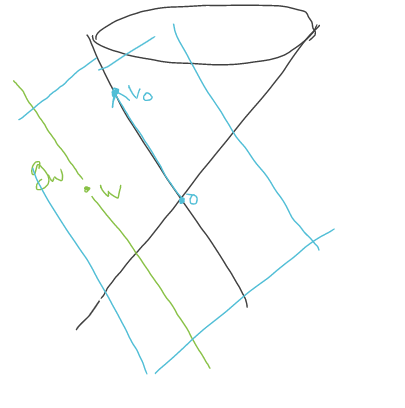
\includegraphics[width=0.5\linewidth]{tangentiale_hyperebene_an_projektive_quadrik}
    \label{fig:tangentiale_hyperebene_an_projektive_quadrik}
  \end{figure}
  \( H \) ist eine Hyperebene. Also \texists \( \rho\in \fieldwithoutzero{K} \) mit
  \begin{equation*}
    \tag{1}s'(v_0,w)=\rho\cdot s(v_0,w)\quad \forall w\in V.\label{teil_bilinearformen_sind_vielfache}
  \end{equation*}
  Nach obigen Überlegungen hat für \( w\in V \) die Gleichung
  \begin{equation*}
    2\lambda s(v_0,w)+q(w)=0
  \end{equation*}
  die gleiche Lösungsmenge wie
  \begin{equation*}
    2\lambda s'(v_0,w)+q'(w)=0.
  \end{equation*}
  Daraus folgt
  \begin{equation*}
    \tag{2}s(v_0,w)q'(w)=s'(v_0,w)q(w)\quad \forall w\in W.\label{bilinearformen_mit_quadriken_vermalung_gleichheit}
  \end{equation*}
  Aus \eqref{bilinearformen_mit_quadriken_vermalung_gleichheit} und \eqref{bilinearformen_mit_quadriken_vermalung_gleichheit} folgt
  \begin{equation*}
    q'(w)=\rho\cdot q(w)\quad \forall w\in V\setminus H.
  \end{equation*}
  Betrachte die Funktion
  \begin{align*}
    h\maps V&\to K\\
    w&\mapsto q'(w)-\rho q(w).
  \end{align*}
  \( h \) it stetig und erfüllt \( \evaluateat{h}{W\setminus H}=0 \). Daraus folgt \( h(w)\quad \forall w\in W \), also \( q'(w)=\rho\cdot q(w)\logicspace \forall w\in V\).

  Für beliebige Vektoren \( v,w\in V \) berechnen wir
  \begin{align*}
    s'(v,w)&=\frac{1}{2}\p*{s'(v+w,v+w)-s'(v,v)-s'(w,w)}\\
    &=\frac{1}{2}(q'(v+w)-q'(v)-q'(w))\\
    &=\frac{1}{2}\tau(q(v+w)-q(v)-q(w))\\
    &=\rho(s(v,w)).
  \end{align*}
\end{proof}
\begin{deferinnerung*}
  Si \( A\in \sqmatrices{n}{\reals} \) eine symmetrische Matrix. Wir definieren die Signatur von \( A \) als
  \begin{equation}
    \begin{split}
      \signature-{A}\definedas \anzahl-{\text{positive Eigenwerte von \( A \)}}-\anzahl-{\text{negative Eigenwerte von \( A \)}}
    \end{split}
  \end{equation}
  (jeweils mit Vielfachheit).
\end{deferinnerung*}
\begin{satz}[Klassifikations-Theorem für reelle und komplexe projektive Quadriken]\label{klassifikation_projektive_quadriken}
  Sei \( K=\reals \) oder \( K=\complexs \) und \( A_1,A_2\in \sqmatrices{(n+1)\times (n+1)}{K} \) symmetrische Matrizen. Definiere
  \begin{equation*}
    Q_i\definedas \Set{(x_0:\dotsc:x_n)\in \projectionspaceover{n}{K}|\transpose{\underline{x}}A_i \underline{x}=0}\logicspace i=1,2.
  \end{equation*}
  \begin{description}
    \item[Fall \( K=\reals \)]
    Die Quadriken \( Q_1 \) und \( Q_2 \) sind geometrisch äquivalent genau dann, wenn
    \begin{equation*}
      \rang-{A_1}=\rang-{A_2}
    \end{equation*}
    und
    \begin{equation*}
      \abs{\signature-{A_1}}=\abs{\signature-{A_2}}.
    \end{equation*}
    \item[Fall \( K=\complexs \)]
    \( Q_1 \) und \( Q_2 \) sind geometrisch äquivalent genau dann, wenn
    \begin{equation*}
      \rang-{A_1}=\rang-{A_2}
    \end{equation*}
  \end{description}
\end{satz}
\begin{korollar}
  Jede Quadrik in \( \projectionspaceover{n}{\reals} \) zu genau einer der Quadriken
  \begin{equation*}
    \Set{(x_0:\dotsb:x_n)\in \projectionspaceover{n}{\reals}|x_0^2+\dotsb+x_k^2-x_{k+1}^2-\dotsb-x_m^2=0}
  \end{equation*}
  mit \( -1\leq \frac{m-1}{2}\leq k\leq m\leq n \) geometrisch äquivalent.

  Jede Quadrik in \( \projectionspaceover{n}{\reals} \) zu genau einer der Quadriken
  \begin{equation*}
    \Set{(x_0:\dotsc:x_n)\in \projectionspaceover{n}{\reals}|x_0^2+\dotsb+x_m^2=0}
  \end{equation*}
  mit \( -1\leq m\leq n \) geometrisch äquivalent.
\end{korollar}
\begin{proof}[Beweis von \thref{klassifikation_projektive_quadriken} für \( K=\reals \)]
  Seien \( A_1,A_2\in\sqmatrices{(n+1)\times (n+1)}{\reals} \) symmetrische Matrizen mit \( \rang-{A_1}=\rang-{A_2} \) und \( \abs{\signature-{A_1}}=\abs{\signature-{A_2}} \). Nach dem Satz über die Hauptachsentransformation reeller symmetrischer Matrizen, existieren \( S_1,S_2\in \invertiblematrices{n+1}{\reals} \) mit  
  \begin{equation*}
    B_i\definedas \transpose{\inverse{S_i}}A_i \inverse{S_i},
  \end{equation*}
  und
  \begin{equation*}
    B_i=\begin{pNiceMatrix} I_{k_i+1} & 0 & 0 \\ 0 & -I_{m_i-k_i} & 0 \\ 0 & 0 & 0 \end{pNiceMatrix}
  \end{equation*}
  wobei \( -1\leq k_i\leq m_i\leq n \) und \( I_l \) die \( l \)-dimensionale Einheitsmatrix ist.

  Nach dem Sylversterschen Trägheitssatz (\aglacourse{1}) folgt
  \begin{equation*}
    m_1+1=\rang-{A_1}=\rang-{A_2}=m_2+1.
  \end{equation*}
  und
  \begin{equation*}
    \abs{2k_1+1-m_1}=\abs{\signature{A_1}}=\abs{\signature{A_2}}=\abs{2k_2+1-m_2}.
  \end{equation*}
  Sei \( m=m_1=m_2 \) und \( k \) gegeben durch
  \begin{equation*}
    2k+1-m=\abs{2k_1+1-m}=2\abs{2k_2+1-m}.
  \end{equation*}
  Dann sind
  \begin{equation*}
    Q_i=\Set{(x_0:\dotsc:x_n)\in \projectionspaceover{n}{\reals}|\transpose{x}A_i\transpose{x}=0}\quad i=1,2
  \end{equation*}
  geometrisch äquivalent zu
  \begin{equation*}
    Q=\Set{(x_0:\dotsc:x_n)\in \projectionspaceover{n}{\reals}|x_0^2+\dotsb+x_k^2-x_{k-1}^2-\dotsb-x_m^2=0}.
  \end{equation*}
  Seien \( Q_1 \), \( Q_2 \) geometrisch äquivalent. Wir können annehmen, dass \( Q_1 \) gegeben ist durch
  \begin{equation*}
    Q_1=\Set{(x_0:\dotsc:x_n)\in \projectionspaceover{n}{\reals}|x_0^2+\dotsb+x_k^2-x_{k+1}^2-\dotsb-x_m^2=0}
  \end{equation*}
  mit \( -1\leq \frac{m-1}{2}\leq k\leq m\leq n \), \dh 
  \begin{equation*}
    Q_1=\Set{(x_0:\dotsc:x_j)\in \projectionspaceover{n}{\reals}|\transpose{\underline{x}}A_1\underline{x}=0}
  \end{equation*}
  mit
  \begin{equation*}
    A_1=\begin{pNiceMatrix} I_{k+1} & 0 & 0 \\ 0 & I_{m-k} & 0 \\ 0 & 0 & 0 \end{pNiceMatrix}.
  \end{equation*}
  Sei 
  \begin{equation*}
    Q_2=\Set{(x_0:\dotsc:x_n)\in\projectionspaceover{n}{\reals}|\transpose{\underline{x}}A_2\underline{x}=0}
  \end{equation*}
  und \( f\maps \projectionspaceover{n}{\reals}\to\projectionspaceover{n}{\reals} \) eine Projektivität mit \( f(Q_2)=Q_1 \). Dann gibt es \( T\in \invertiblematrices{n+1}{\reals} \), sodass
  \begin{equation*}
    f(Q_2)=\Set{(x_0:\dotsc:x_n)\in \projectionspaceover{n}{\reals}|\transpose{\underline{x}}\transpose{T}A_2T \underline{x}=0}.
  \end{equation*}
  Sei \( A'\definedas \transpose{T}A_2 T \). Sei \( k\neq m \). Dann ist \( 0\leq k<m \) und die Vektoren
  \begin{align*}
    v_0&\definedas (\braceannotate{m \text{ Einträge}{1,0,\dotsc,n},1,0,\dotsc,0})\\
    w&\definedas(1,0,\dotsc,0)
  \end{align*}
  erfüllen
  \begin{equation*}
    \transpose{v_0}A_1 v_0=0\quad \transpose{v_0}A_1 w=1.
  \end{equation*}
  Aus \thref{gleicher_kegel_bilinearformen_vielfache_kriterium} folgt, dass
  \begin{equation*}
    A'=\rho A_1\quad \rho\in \fieldwithoutzero{\reals}.
  \end{equation*}
  Es ist
  \begin{align*}
    \rang-{A'}&=\rang{A_1}\\
    \abs{\signature-{A'}}&=\abs{\signature-{A_1}}
  \end{align*}
  und nach dem Sylversterschen Trägheitsgesetz folgt
  \begin{equation*}
    \rang-{A_2}=\rang-{A'}=\rang-{A_1}
  \end{equation*}
  und
  \begin{equation*}
    \abs{\signature-{A_2}}=\abs{\signature-{A'}}=\abs{\signature-{A_1}}.
  \end{equation*}
  Sei \( k=m \), also
  \begin{align*}
    Q_1&=\Set{(x_0:\dotsb:x_n)\in \projectionspaceover{n}{\reals}|x_0^2+\dotsb+x_m^2=0}\\
    &=\Set{(x_0:\dotsc:x_n)\in \projectionspaceover{n}{\reals}|x_0=\dotsb=x_m=0}
  \end{align*}
  projektiver Unterraum der Dimension \( n-m-1 \). Also ist auch \( f(Q_2) \) projektiver Unterraum der Dimension \( n-m-1 \). Daraus folgt
  \begin{equation*}
    \rang{A'}=\abs{\signature-{A'}}=m+1
  \end{equation*}
  und nach dem Sylversterschen Trägheitsgesetz
  \begin{align*}
    \rang-{A_2}&=\rang-{A'}=m+1=\rang-{A_1}\\
    \abs{\signature-{A_2}}=\abs{\signature-{A'}}=m+1=\abs{\signature-{A_1}}.
  \end{align*}
\end{proof}
